% Source reference: :contentReference[oaicite:0]{index=0}
\part{Graph Theory}
\section{Handout 11: Graph Theory (5): Minimum Spanning Trees, Shortest Paths}

\subsection{Overview}

This handout is the final graph-theory handout. It focuses on two weighted-graph optimisation problems:
\begin{itemize}[leftmargin=*]
    \item \emph{minimum spanning tree} problems: connect all vertices with minimum total edge weight;
    \item \emph{shortest path} problems: find minimum-weight routes between vertices.
\end{itemize}

The main algorithms are:
\[
\text{Kruskal's Algorithm},
\qquad
\text{Prim's Algorithm},
\qquad
\text{Dijkstra's Algorithm}.
\]

The central distinction is:
\[
\text{MST: choose edges to connect all vertices}
\qquad\text{versus}\qquad
\text{Shortest path: choose a route between vertices}.
\]

\begin{examtip}[title={Main diagnostic for Handout 11}]
Before applying an algorithm, identify the objective:
\[
\begin{array}{c|c}
\text{Objective} & \text{Relevant method} \\ \hline
\text{connect all vertices with minimum total weight} & \text{MST: Kruskal / Prim} \\
\text{shortest route from one source to one target} & \text{Dijkstra until target settled} \\
\text{shortest routes from one source to all vertices} & \text{full Dijkstra}
\end{array}
\]
Do not use MST algorithms to solve shortest-path problems, and do not use shortest-path algorithms to build MSTs.
\end{examtip}

%==================================================
\subsection{Algorithms}
%==================================================

\begin{definition}{Algorithm}{algorithm-def}
An \emph{algorithm} is a finite mechanical procedure that starts with an input and produces an output after executing a sequence of well-defined primitive steps.
\end{definition}

Two basic criteria for judging an algorithm are:
\begin{itemize}[leftmargin=*]
    \item \emph{correctness}: the algorithm always returns the desired output;
    \item \emph{running time}: the number of primitive steps needed as a function of input size.
\end{itemize}

\begin{examtip}[title={How algorithms are assessed in this handout}]
The lecture emphasises correctness ideas more than detailed complexity analysis. For MST algorithms, correctness is based on safe edges and cut arguments. For Dijkstra's algorithm, correctness is based on settling vertices in increasing distance from the source.
\end{examtip}

%==================================================
\subsection{Recall: Spanning Trees and Minimum Spanning Trees}
%==================================================

\begin{definition}{Spanning tree}{spanning-tree-recall}
Let \(G=(V,E)\) be a connected simple graph. A \emph{spanning tree} of \(G\) is a subgraph \(T\) of \(G\) such that:
\begin{itemize}[leftmargin=*]
    \item \(T\) is a tree;
    \item \(V(T)=V(G)\).
\end{itemize}
\end{definition}

\begin{definition}{Minimum spanning tree}{mst-def}
Let \(G=(V,E,W)\) be a connected edge-weighted graph, where
\[
W:E\to \mathbb{R}
\]
assigns a weight or cost to each edge. A \emph{minimum spanning tree}, abbreviated MST, is a spanning tree \(T\) of \(G\) whose total weight
\[
W(T)=\sum_{e\in E(T)}W(e)
\]
is as small as possible among all spanning trees of \(G\).
\end{definition}

\begin{keyformula}[title={MST objective}]
\[
\text{minimize }
\sum_{e\in E(T)}W(e)
\qquad
\text{over all spanning trees }T\text{ of }G.
\]
\end{keyformula}

\begin{examplebox}[title={What an MST must satisfy}]
If \(G\) is connected and has \(n\) vertices, then every MST:
\begin{itemize}[leftmargin=*]
    \item contains all \(n\) vertices;
    \item has exactly \(n-1\) edges;
    \item is connected;
    \item contains no cycle;
    \item has minimum total weight among all spanning trees.
\end{itemize}
\end{examplebox}

\begin{commonmistake}[title={MST is not usually a shortest-path tree}]
A minimum spanning tree minimizes the \emph{total} weight needed to connect all vertices. It does not necessarily preserve the shortest path from a chosen source to every other vertex.
\end{commonmistake}

%==================================================
\subsection{Greedy Approach to MST}
%==================================================

Both Kruskal's and Prim's algorithms are greedy algorithms. At each step, they make a locally cheapest choice that is guaranteed to be safe.

A generic MST greedy algorithm has the form:
\[
\begin{array}{l}
T\leftarrow \varnothing;\\
\text{while }T\text{ is not a spanning tree:}\\
\qquad \text{choose an edge }e\text{ satisfying a safe condition};\\
\qquad T\leftarrow T\cup\{e\};\\
\text{return }T.
\end{array}
\]

The key mathematical question is:

\begin{center}
\emph{Which locally cheap edges are guaranteed to belong to an MST?}
\end{center}

This is answered by the cut property.

\begin{examtip}[title={Greedy algorithms need proof}]
A greedy choice is not correct merely because it is cheap. The proof must show that the chosen edge can safely belong to an MST.
\end{examtip}

%==================================================
\subsection{Cuts and Safe Edges}
%==================================================

\begin{definition}{Cut}{cut-def}
Let \(G=(V,E)\) be a graph. A \emph{cut} is a partition of \(V\) into two disjoint nonempty subsets
\[
S
\qquad\text{and}\qquad
V\setminus S.
\]
An edge \(\{u,v\}\in E\) \emph{crosses the cut} if one endpoint lies in \(S\) and the other lies in \(V\setminus S\).
\end{definition}

% Cut diagram showing vertices split into S and V\S with crossing edges.
\begin{center}
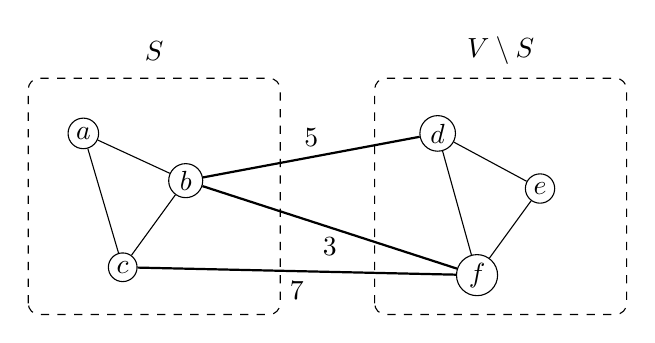
\begin{tikzpicture}[scale=1.0]
    \draw[dashed,rounded corners] (-1.2,-1.5) rectangle (2.0,1.5);
    \draw[dashed,rounded corners] (3.2,-1.5) rectangle (6.4,1.5);
    \node at (0.4,1.85) {\(S\)};
    \node at (4.8,1.85) {\(V\setminus S\)};

    \node[circle,draw,inner sep=1.5pt] (a) at (-0.5,0.8) {\(a\)};
    \node[circle,draw,inner sep=1.5pt] (b) at (0.8,0.2) {\(b\)};
    \node[circle,draw,inner sep=1.5pt] (c) at (0.0,-0.9) {\(c\)};

    \node[circle,draw,inner sep=1.5pt] (d) at (4.0,0.8) {\(d\)};
    \node[circle,draw,inner sep=1.5pt] (e) at (5.3,0.1) {\(e\)};
    \node[circle,draw,inner sep=1.5pt] (f) at (4.5,-1.0) {\(f\)};

    \draw (a)--(b)--(c)--(a);
    \draw (d)--(e)--(f)--(d);
    \draw[thick] (b)--node[above]{\(5\)}(d);
    \draw[thick] (b)--node[below]{\(3\)}(f);
    \draw[thick] (c)--node[below]{\(7\)}(f);
\end{tikzpicture}
\end{center}

\begin{definition}{Safe edge}{safe-edge}
Assume the edge costs in a connected undirected graph are distinct. An edge \(e\) is called a \emph{safe edge} if there exists a cut
\[
(S,V\setminus S)
\]
such that \(e\) is the unique minimum-cost edge crossing that cut.
\end{definition}

\begin{theorem}{Cut property}{cut-property}
Assume \(G\) is a connected undirected graph with distinct edge costs. Then every safe edge belongs to every minimum spanning tree of \(G\).
\end{theorem}

\begin{proof}
Let \(e=\{u,v\}\) be safe for the cut \((S,V\setminus S)\), and suppose for contradiction that some MST \(T\) does not contain \(e\).

Adding \(e\) to \(T\) creates a unique cycle. Since \(e\) crosses the cut, the cycle must contain another edge \(e'\) that also crosses the same cut. Because \(e\) is the unique minimum-cost edge crossing the cut,
\[
W(e)<W(e').
\]
Now replace \(e'\) by \(e\):
\[
T'=(T\setminus\{e'\})\cup\{e\}.
\]
The graph \(T'\) is still a spanning tree, but
\[
W(T')=W(T)-W(e')+W(e)<W(T),
\]
contradicting that \(T\) is an MST. Therefore every MST contains \(e\).
\end{proof}

\begin{theorem}{Safe edges form the unique MST under distinct costs}{safe-edges-mst}
Assume \(G\) is connected and all edge costs are distinct. Then the set of all safe edges forms the unique minimum spanning tree of \(G\).
\end{theorem}

\begin{proof}
By the cut property, every safe edge belongs to every MST.

It remains to see that the safe edges connect all vertices. Suppose the graph formed by the safe edges is not connected. Let \(S\) be the vertex set of one of its connected components. Since \(G\) is connected, at least one edge of \(G\) crosses the cut \((S,V\setminus S)\). Because edge costs are distinct, there is a unique minimum-cost edge crossing this cut. By definition, that edge is safe, but then it would connect \(S\) to \(V\setminus S\), contradicting that \(S\) was a component of the safe-edge graph.

Hence the safe edges form a connected spanning subgraph. Since every safe edge belongs to every MST and an MST has exactly \(n-1\) edges, these safe edges are exactly the unique MST.
\end{proof}

\begin{extension}[title={Why distinct costs simplify the theory}]
Distinct edge costs ensure that each cut has a unique cheapest crossing edge. Without distinct costs, MSTs may not be unique, but Kruskal's and Prim's algorithms still produce an MST when ties are handled arbitrarily.
\end{extension}

%==================================================
\subsection{Kruskal's Algorithm}
%==================================================

Kruskal's algorithm grows a forest. It processes edges globally from cheapest to most expensive and adds an edge exactly when it does not create a cycle.

\begin{theorem}{Kruskal's Algorithm}{kruskal-algorithm}
Given a connected undirected edge-weighted graph \(G=(V,E,W)\):
\[
\begin{array}{l}
T\leftarrow \varnothing;\\
\text{sort edges in increasing order of weight;}\\
\text{for each edge }e\text{ in this order:}\\
\qquad \text{if }T\cup\{e\}\text{ contains no cycle, then }T\leftarrow T\cup\{e\};\\
\qquad \text{stop once }|T|=|V|-1;\\
\text{return }T.
\end{array}
\]
The returned graph \(T\) is a minimum spanning tree.
\end{theorem}

\begin{proof}
At every stage, \(T\) is a forest. Suppose Kruskal adds an edge \(e=\{u,v\}\). Let \(S\) be the vertex set of the connected component of \(T\) containing \(u\) just before \(e\) is added. Since \(e\) does not form a cycle, \(v\notin S\), so \(e\) crosses the cut \((S,V\setminus S)\).

Any cheaper edge crossing this cut would also connect two different components at the time it was considered, and hence would have been added earlier. Therefore \(e\) is the cheapest edge crossing this cut. Under distinct costs, it is the unique cheapest crossing edge, so it is safe.

Thus every edge added by Kruskal is safe and hence belongs to the MST. The algorithm stops after adding \(n-1\) edges without forming a cycle, so the result is a spanning tree. Since all its edges are safe, it is the MST.
\end{proof}

\begin{keyformula}[title={Kruskal's rule}]
\[
\text{Process edges by increasing weight; add the next edge iff it does not create a cycle.}
\]
\end{keyformula}

\begin{examplebox}[title={Kruskal example}]
Let \(G\) have vertices
\[
\{a,b,c,d,e\}
\]
and weighted edges
\[
ab:1,\quad bc:2,\quad ac:3,\quad bd:4,\quad cd:5,\quad de:6,\quad ce:7.
\]
Process edges in increasing order:
\[
ab,\ bc,\ ac,\ bd,\ cd,\ de,\ ce.
\]
Kruskal adds:
\[
ab,\quad bc,
\]
then skips \(ac\) because \(ab,bc,ac\) would form a cycle. It then adds
\[
bd,\quad de.
\]
Now there are \(5-1=4\) edges, so the algorithm stops. The MST is
\[
\{ab,bc,bd,de\}
\]
with total weight
\[
1+2+4+6=13.
\]
\end{examplebox}

\begin{commonmistake}[title={Kruskal is not ``choose the cheapest adjacent edge''}]
Kruskal does not grow one connected tree from a starting vertex. It may maintain several components at once. Its only rule is global increasing edge order plus the no-cycle test.
\end{commonmistake}

%==================================================
\subsection{Prim's Algorithm}
%==================================================

Prim's algorithm grows one tree. It starts from a vertex and repeatedly attaches the cheapest edge from the current tree to a new vertex.

\begin{theorem}{Prim's Algorithm}{prim-algorithm}
Given a connected undirected edge-weighted graph \(G=(V,E,W)\), choose a starting vertex \(s\). Then:
\[
\begin{array}{l}
T\leftarrow \varnothing;\\
S\leftarrow \{s\};\\
\text{while }S\neq V:\\
\qquad \text{choose a minimum-weight edge }e=\{u,v\}\\
\qquad \text{with }u\in S\text{ and }v\in V\setminus S;\\
\qquad T\leftarrow T\cup\{e\};\\
\qquad S\leftarrow S\cup\{v\};\\
\text{return }T.
\end{array}
\]
The returned graph \(T\) is a minimum spanning tree.
\end{theorem}

\begin{proof}
At each step, \(S\) is the vertex set of the tree currently built by the algorithm. The edge chosen by Prim is the minimum-weight edge crossing the cut
\[
(S,V\setminus S).
\]
Under distinct costs, it is the unique minimum crossing edge, so it is safe by the cut property. Therefore every edge added belongs to the MST.

Each iteration adds exactly one new vertex to \(S\), so the algorithm eventually reaches \(S=V\). The selected edges connect all vertices and contain no cycle because each new edge attaches one new vertex. Hence the output is a spanning tree made of safe edges, and therefore is the MST.
\end{proof}

\begin{keyformula}[title={Prim's rule}]
\[
\text{Grow one tree; repeatedly add the cheapest edge crossing from the tree to outside.}
\]
\end{keyformula}

\begin{examplebox}[title={Prim example on the same graph}]
Using the graph from the Kruskal example and starting at \(a\):
\[
ab:1,\quad bc:2,\quad ac:3,\quad bd:4,\quad cd:5,\quad de:6,\quad ce:7.
\]
Start with
\[
S=\{a\}.
\]
The cheapest edge leaving \(S\) is \(ab\), so add \(b\):
\[
S=\{a,b\}.
\]
The cheapest edge leaving \(S\) is \(bc\), so add \(c\):
\[
S=\{a,b,c\}.
\]
The cheapest edge leaving \(S\) is \(bd\), so add \(d\):
\[
S=\{a,b,c,d\}.
\]
Finally the cheapest edge leaving \(S\) is \(de\), so add \(e\). The MST is again
\[
\{ab,bc,bd,de\},
\]
with total weight \(13\).
\end{examplebox}

\begin{examtip}[title={Kruskal versus Prim}]
\[
\begin{array}{c|c}
\text{Kruskal} & \text{global edge order; avoids cycles} \\
\text{Prim} & \text{one growing tree; crosses the current cut}
\end{array}
\]
Both rely on the same cut-property idea.
\end{examtip}

%==================================================
\subsection{Shortest Paths in Weighted Graphs}
%==================================================

\begin{definition}{Weighted graph and path length}{weighted-path}
Let \(G=(V,E,W)\) be an edge-weighted graph. If an edge \(e=(u,v)\) has weight
\[
\ell(e)=\ell(u,v),
\]
then the \emph{length} of a path is the sum of the weights of all edges on the path.
\end{definition}

\begin{definition}{Shortest path and distance}{shortest-path-distance}
Let \(u,v\in V\). A \emph{shortest path} from \(u\) to \(v\) is a simple path from \(u\) to \(v\) whose total length is minimum among all paths from \(u\) to \(v\).

The \emph{distance} from \(u\) to \(v\), denoted \(d(u,v)\), is the length of a shortest path from \(u\) to \(v\). If no path connects \(u\) to \(v\), then
\[
d(u,v)=\infty.
\]
\end{definition}

In this handout, shortest-path algorithms are studied for graphs with \emph{non-negative} edge lengths.

\begin{examplebox}[title={Shortest path interpretation}]
If vertices represent MRT stations or road junctions, and edge weights represent travel time or distance, then a shortest path represents a route of minimum total travel cost.
\end{examplebox}

\begin{commonmistake}[title={Fewest edges need not mean shortest path}]
A path with fewer edges may have larger total weight than a path with more edges. Shortest path means minimum total edge weight, not minimum number of edges.
\end{commonmistake}

\subsubsection{Types of shortest-path problems}

Typical shortest-path problems include:
\begin{enumerate}[leftmargin=*]
    \item \emph{single-pair shortest path}: given \(s,t\), find a shortest path from \(s\) to \(t\);
    \item \emph{single-source shortest paths}: given \(s\), find shortest paths from \(s\) to all vertices;
    \item \emph{all-pairs shortest paths}: find shortest paths between all pairs of vertices.
\end{enumerate}

This handout focuses mainly on the first two. For undirected graphs, each undirected edge may be replaced by two directed edges of the same weight, one in each direction.

% Directed replacement of an undirected weighted edge.
\begin{center}
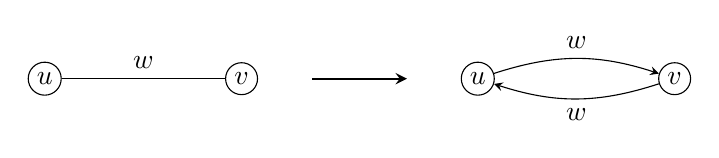
\begin{tikzpicture}[>=stealth,scale=1.0]
    \node[circle,draw,inner sep=1.7pt] (u1) at (0,0) {\(u\)};
    \node[circle,draw,inner sep=1.7pt] (v1) at (2.5,0) {\(v\)};
    \draw (u1)--node[above]{\(w\)}(v1);

    \draw[->,thick] (3.4,0)--(4.6,0);

    \node[circle,draw,inner sep=1.7pt] (u2) at (5.5,0) {\(u\)};
    \node[circle,draw,inner sep=1.7pt] (v2) at (8.0,0) {\(v\)};
    \draw[->,bend left=18] (u2) to node[above]{\(w\)} (v2);
    \draw[->,bend left=18] (v2) to node[below]{\(w\)} (u2);
\end{tikzpicture}
\end{center}

%==================================================
\subsection{Shortest Path Structure}
%==================================================

The correctness of Dijkstra's algorithm rests on two structural facts.

\begin{theorem}{Subpaths of shortest paths are shortest}{shortest-subpath}
Let
\[
s=v_0\to v_1\to\cdots\to v_k=v
\]
be a shortest path from \(s\) to \(v\). Then for every \(1\le i<k\), the subpath
\[
s=v_0\to v_1\to\cdots\to v_i
\]
is a shortest path from \(s\) to \(v_i\).
\end{theorem}

\begin{proof}
Suppose the subpath from \(s\) to \(v_i\) were not shortest. Then there would be another path from \(s\) to \(v_i\) with smaller total length. Replacing the original initial segment by this shorter path would produce a path from \(s\) to \(v\) shorter than the original path, contradicting that the original path was shortest.
\end{proof}

\begin{theorem}{Next closest vertex principle}{next-closest}
Suppose \(S\) contains the already-settled vertices closest to a source \(s\). If \(u\notin S\) is the next closest vertex to \(s\), then a shortest path from \(s\) to \(u\) reaches \(u\) by one final edge from some vertex in \(S\).
\end{theorem}

\begin{proof}
Let
\[
P:s=v_0\to v_1\to\cdots\to v_k=u
\]
be a shortest path from \(s\) to \(u\). Every intermediate vertex \(v_i\), with \(i<k\), has distance
\[
d(s,v_i)<d(s,u)
\]
when edge lengths are non-negative and the path is simple. Therefore each such intermediate vertex is already among the closer settled vertices in \(S\). In particular, the predecessor \(v_{k-1}\) of \(u\) lies in \(S\), and the last step is an edge from \(S\) to \(u\).
\end{proof}

\begin{extension}[title={Why non-negative weights matter}]
Dijkstra's algorithm relies on the fact that extending a path cannot reduce its length. Negative edge weights can invalidate the claim that once a vertex is chosen as closest, its distance is final.
\end{extension}

%==================================================
\subsection{Tentative Distances and Relaxation}
%==================================================

Let \(s\) be the source vertex. For each vertex \(v\), Dijkstra's algorithm maintains a tentative distance \(d(v)\).

\begin{definition}{Relaxation}{relaxation}
Given a directed edge \((u,v)\) with length \(\ell(u,v)\), \emph{relaxing} the edge means replacing
\[
d(v)
\]
by
\[
\min\{d(v),\,d(u)+\ell(u,v)\}.
\]
\end{definition}

The idea is that if the best known path to \(u\) has length \(d(u)\), then travelling from \(u\) to \(v\) gives a candidate path to \(v\) of length
\[
d(u)+\ell(u,v).
\]

\begin{keyformula}[title={Relaxation update}]
\[
d(v)\leftarrow \min\{d(v),\,d(u)+\ell(u,v)\}.
\]
\end{keyformula}

% Relaxation diagram showing a candidate improvement from u to v.
\begin{center}
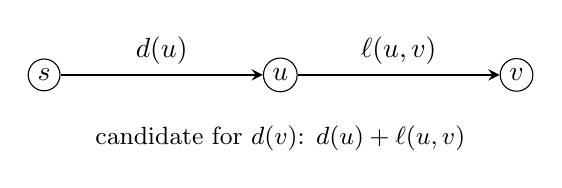
\begin{tikzpicture}[>=stealth,scale=1.0]
    \node[circle,draw,inner sep=1.8pt] (s) at (0,0) {\(s\)};
    \node[circle,draw,inner sep=1.8pt] (u) at (3,0) {\(u\)};
    \node[circle,draw,inner sep=1.8pt] (v) at (6,0) {\(v\)};

    \draw[->,thick] (s)--node[above]{\(d(u)\)}(u);
    \draw[->,thick] (u)--node[above]{\(\ell(u,v)\)}(v);

    \node at (3,-0.8) {\small candidate for \(d(v)\): \(d(u)+\ell(u,v)\)};
\end{tikzpicture}
\end{center}

\begin{examtip}[title={Relaxation is the atomic step of Dijkstra}]
Every update in Dijkstra's algorithm is a relaxation of an outgoing edge from the newly settled vertex.
\end{examtip}

%==================================================
\subsection{Dijkstra's Algorithm}
%==================================================

\begin{theorem}{Dijkstra's Algorithm}{dijkstra-algorithm}
Let \(G=(V,E)\) be a directed weighted graph with non-negative edge lengths, and let \(s\in V\). Dijkstra's algorithm computes the shortest-path distance from \(s\) to every vertex reachable from \(s\):
\[
\begin{array}{l}
\text{for every }v\in V,\ d(v)\leftarrow \infty;\\
d(s)\leftarrow 0;\\
S\leftarrow \varnothing;\\[0.2em]
\text{while }S\neq V:\\
\qquad \text{choose }u\in V\setminus S\text{ with minimum }d(u);\\
\qquad S\leftarrow S\cup\{u\};\\
\qquad \text{for each edge }(u,v)\text{ with }v\notin S:\\
\qquad\qquad d(v)\leftarrow \min\{d(v),d(u)+\ell(u,v)\};\\
\text{return the values }d(v).
\end{array}
\]
\end{theorem}

\begin{proof}
We prove by induction on the number of iterations that whenever a vertex \(u\) is added to \(S\), the value \(d(u)\) equals the true shortest distance from \(s\) to \(u\).

Initially, \(d(s)=0\), and no other vertex can have distance less than \(0\) because edge lengths are non-negative.

Assume the claim holds for all vertices already in \(S\). Let \(u\in V\setminus S\) be chosen with minimum tentative distance. Suppose, for contradiction, that there is a shorter path \(P\) from \(s\) to \(u\) than \(d(u)\). Along \(P\), let \(y\) be the first vertex not in \(S\), and let \(x\) be the vertex immediately before \(y\). Then \(x\in S\).

By the induction hypothesis, \(d(x)\) is already the true shortest distance to \(x\). When \(x\) was added to \(S\), the edge \((x,y)\) was relaxed, so
\[
d(y)\le d(x)+\ell(x,y).
\]
The portion of \(P\) from \(s\) to \(y\) is no longer than the full path \(P\) from \(s\) to \(u\), because edge lengths are non-negative. Thus \(d(y)\) is less than the alleged shorter length to \(u\), and hence less than \(d(u)\). But \(u\) was chosen as the vertex outside \(S\) with minimum tentative distance, a contradiction.

Therefore \(d(u)\) is final when \(u\) is added to \(S\). By induction, the algorithm is correct.
\end{proof}

\begin{keyformula}[title={Dijkstra invariant}]
Once a vertex enters \(S\), its tentative value \(d(v)\) is final:
\[
v\in S
\quad\Longrightarrow\quad
d(v)=\text{true shortest distance from }s\text{ to }v.
\]
\end{keyformula}

\begin{commonmistake}[title={Dijkstra is not valid for negative edge lengths}]
The correctness proof uses non-negative edge lengths. If negative edges are allowed, a vertex that appears settled may later be improved through a negative edge.
\end{commonmistake}

%==================================================
\subsection{Worked Dijkstra Example}
%==================================================

Consider the directed weighted graph with vertices
\[
\{a,b,c,d,e,z\}
\]
and directed edges
\[
a\to b:4,\quad a\to c:2,\quad c\to b:1,\quad c\to d:8,\quad c\to e:10,
\]
\[
b\to d:5,\quad d\to e:2,\quad d\to z:6,\quad e\to z:3.
\]

% Directed weighted graph for Dijkstra example.
\begin{center}
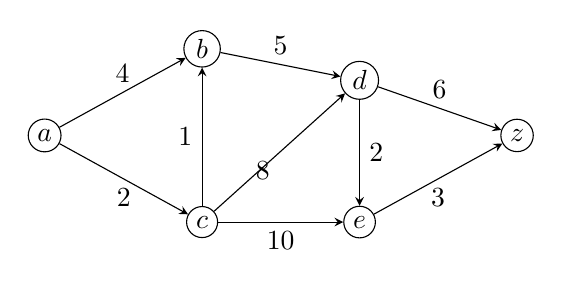
\begin{tikzpicture}[>=stealth,scale=1.0]
    \node[circle,draw,inner sep=1.8pt] (a) at (0,0) {\(a\)};
    \node[circle,draw,inner sep=1.8pt] (c) at (2,-1.1) {\(c\)};
    \node[circle,draw,inner sep=1.8pt] (b) at (2,1.1) {\(b\)};
    \node[circle,draw,inner sep=1.8pt] (d) at (4,0.7) {\(d\)};
    \node[circle,draw,inner sep=1.8pt] (e) at (4,-1.1) {\(e\)};
    \node[circle,draw,inner sep=1.8pt] (z) at (6,0) {\(z\)};

    \draw[->] (a)--node[above]{\(4\)}(b);
    \draw[->] (a)--node[below]{\(2\)}(c);
    \draw[->] (c)--node[left]{\(1\)}(b);
    \draw[->] (b)--node[above]{\(5\)}(d);
    \draw[->] (c)--node[below left]{\(8\)}(d);
    \draw[->] (c)--node[below]{\(10\)}(e);
    \draw[->] (d)--node[right]{\(2\)}(e);
    \draw[->] (d)--node[above]{\(6\)}(z);
    \draw[->] (e)--node[below]{\(3\)}(z);
\end{tikzpicture}
\end{center}

\begin{examplebox}[title={Dijkstra from source \(a\)}]
Initialize
\[
d(a)=0,\qquad d(b)=d(c)=d(d)=d(e)=d(z)=\infty,
\qquad S=\varnothing.
\]

The successive table of tentative distances is:
\[
\begin{array}{c|cccccc|c}
\text{Round} & d(a)&d(b)&d(c)&d(d)&d(e)&d(z)&S\\ \hline
0 &0&\infty&\infty&\infty&\infty&\infty&\varnothing\\
1 &0&4&2&\infty&\infty&\infty&\{a\}\\
2 &0&3&2&10&12&\infty&\{a,c\}\\
3 &0&3&2&8&12&\infty&\{a,c,b\}\\
4 &0&3&2&8&10&14&\{a,c,b,d\}\\
5 &0&3&2&8&10&13&\{a,c,b,d,e\}\\
6 &0&3&2&8&10&13&\{a,c,b,d,e,z\}.
\end{array}
\]

Thus the final shortest-path distances from \(a\) are:
\[
d(a)=0,\quad d(c)=2,\quad d(b)=3,\quad d(d)=8,\quad d(e)=10,\quad d(z)=13.
\]
\end{examplebox}

\begin{extension}[title={Recovering actual shortest paths}]
To recover the shortest path itself, not just its length, store a predecessor each time a relaxation improves \(d(v)\). For example, if \(d(v)\) is improved using \(u\to v\), set
\[
\operatorname{pred}(v)=u.
\]
Tracing predecessors backward from the target reconstructs the shortest path.
\end{extension}

%==================================================
\subsection{Shortest Path Algorithm with \(\pi\)-Values}
%==================================================

The handout first presents Dijkstra's idea using values
\[
\pi(u)=\min_{a\in S}\{d(a)+\ell(a,u)\}
\]
for unexplored vertices \(u\notin S\). Here \(S\) is the set of vertices whose shortest distances have already been determined.

\begin{theorem}{\(\pi\)-value selection rule}{pi-selection-rule}
Assume \(S\) contains the already settled vertices. For \(u\in V\setminus S\), define
\[
\pi(u)=\min_{a\in S}\{d(a)+\ell(a,u)\}.
\]
Then the next closest vertex to \(s\) is a vertex \(u\in V\setminus S\) minimizing \(\pi(u)\).
\end{theorem}

\begin{proof}
By the next closest vertex principle, a shortest path to the next closest unsettled vertex enters it from some settled vertex \(a\in S\). Thus its distance is of the form
\[
d(a)+\ell(a,u)
\]
for some \(a\in S\), and the best such value is \(\pi(u)\). Therefore the next closest vertex is obtained by minimizing \(\pi(u)\) over all vertices outside \(S\).
\end{proof}

The efficient implementation stores these \(\pi\)-values directly as the tentative distances \(d(v)\). When a new vertex \(u\) is settled, only edges leaving \(u\) need to be scanned.

\begin{examtip}[title={Why the optimized update is enough}]
Since \(S\) only grows, the only new possible shortest route to an unsettled vertex \(v\) after adding \(u\) is a route that enters \(v\) through \(u\). Hence the update
\[
d(v)\leftarrow \min\{d(v),d(u)+\ell(u,v)\}
\]
is sufficient.
\end{examtip}

%==================================================
\subsection{MST versus Shortest Path Trees}
%==================================================

Both MST and shortest-path algorithms output trees in many situations, but the objectives are different.

\begin{center}
\small
\begin{tabular}{@{}p{0.24\textwidth}p{0.31\textwidth}p{0.33\textwidth}@{}}
\toprule
\textbf{Object} & \textbf{Objective} & \textbf{Typical algorithm} \\
\midrule
Minimum spanning tree & minimize total cost of connecting all vertices & Kruskal / Prim \\
Shortest path tree from \(s\) & minimize distance from \(s\) to each vertex & Dijkstra \\
\bottomrule
\end{tabular}
\end{center}

\begin{examplebox}[title={Different objectives can give different trees}]
A spanning tree of small total weight may give a long route between two particular vertices. Conversely, the union of shortest paths from a source may have larger total weight than an MST. Therefore the two problems should be treated separately.
\end{examplebox}

%==================================================
\subsection{Special Techniques}
%==================================================

\subsubsection*{1. Use cut arguments for MST correctness}
To prove an edge is safe, find a cut for which that edge is the unique cheapest crossing edge.

\subsubsection*{2. For Kruskal, track components}
Kruskal's algorithm is easiest to execute by maintaining connected components. Add an edge exactly when its endpoints lie in different components.

\subsubsection*{3. For Prim, track the growing vertex set}
Prim's algorithm is easiest to execute by maintaining the current vertex set \(S\). Add the cheapest edge crossing from \(S\) to \(V\setminus S\).

\subsubsection*{4. For Dijkstra, maintain settled and unsettled vertices}
The settled set \(S\) contains vertices whose shortest distances are final. Always choose the unsettled vertex with smallest tentative distance.

\subsubsection*{5. Relax outgoing edges systematically}
After settling \(u\), update every outgoing neighbour \(v\) using
\[
d(v)\leftarrow \min\{d(v),d(u)+\ell(u,v)\}.
\]

\subsubsection*{6. Stop early for a single target}
If the goal is only to find a shortest path from \(s\) to \(t\), Dijkstra can stop once \(t\) is added to \(S\).

\subsubsection*{7. Check assumptions before using an algorithm}
For MST algorithms, the graph should be connected and undirected. For Dijkstra in this handout, edge lengths must be non-negative.

\begin{extension}[title={Unified greedy viewpoint}]
Kruskal, Prim, and Dijkstra are all greedy, but their invariants differ:
\[
\begin{array}{c|c}
\text{Algorithm} & \text{Invariant} \\ \hline
\text{Kruskal} & T\text{ is a forest of safe edges} \\
\text{Prim} & T\text{ is one tree of safe edges} \\
\text{Dijkstra} & S\text{ contains vertices with finalized shortest distances}
\end{array}
\]
Remembering the invariant prevents mixing the algorithms.
\end{extension}

%==================================================
\subsection{Summary Table}
%==================================================

\begin{center}
\small
\begin{tabular}{@{}p{0.25\textwidth}p{0.31\textwidth}p{0.33\textwidth}@{}}
\toprule
\textbf{Concept} & \textbf{Definition / rule} & \textbf{Exam use} \\
\midrule
Spanning tree & tree subgraph containing all vertices & connects graph minimally by edges \\
MST & spanning tree of minimum total weight & optimal network design \\
Cut & partition \((S,V\setminus S)\) & isolates crossing edges \\
Safe edge & unique minimum edge crossing some cut & belongs to every MST under distinct costs \\
Cut property & safe edges are in every MST & correctness of MST algorithms \\
Kruskal & add edges in increasing weight if no cycle forms & MST by global edge order \\
Prim & repeatedly add cheapest edge crossing current cut & MST by growing one tree \\
Path length & sum of edge weights on a path & weighted route cost \\
Distance & length of a shortest path, or \(\infty\) if unreachable & shortest-path value \\
Relaxation & \(d(v)\leftarrow\min\{d(v),d(u)+\ell(u,v)\}\) & Dijkstra update step \\
Dijkstra & settle vertices in increasing tentative distance & single-source shortest paths \\
\bottomrule
\end{tabular}
\end{center}

\begin{examtip}[title={Final checklist for Handout 11}]
Before finalizing a solution, check:
\begin{enumerate}[leftmargin=*]
    \item Is the problem asking for an MST or a shortest path?
    \item For an MST problem, have you avoided cycles while connecting all vertices?
    \item For Kruskal, did you process edges in increasing order?
    \item For Prim, did you choose the cheapest edge crossing from the current tree?
    \item For Dijkstra, are all edge weights non-negative?
    \item After each Dijkstra step, did you relax outgoing edges from the newly settled vertex?
    \item If a vertex remains at distance \(\infty\), is it unreachable from the source?
\end{enumerate}
\end{examtip}

\begin{commonmistake}[title={Final warning for Handout 11}]
Kruskal, Prim, and Dijkstra are all greedy algorithms, but they solve different optimisation problems. Kruskal and Prim minimize total spanning-tree weight; Dijkstra minimizes distances from a source.
\end{commonmistake}